\chapter{Security-constrained optimal power flow (\scopflow)}\label{chap:scopflow}
SCOPFLOW solves a contingency-constrained optimal power flow problem. The problem is set up as a two-stage optimization problem where the first-stage (base-case) represents the normal operation of the grid and the second-stage comprises $N_c$ contingency scenarios. Each contingency scenario can be single or multi-period.

\section{Formulation}

\subsection{Single-period}

The contingency-constrained optimal power flow (popularly termed as security-constrained optimal power flow (SCOPF) in power system parlance) attempts to find a least cost dispatch for the base case (or no contingency) while ensuring that if any of contingencies do occur then the system will be secure. This is illustrated in Fig. \ref{fig:scopflow} for a SCOPF with a base-case $c_0$ and three contingencies.

\definecolor{lavander}{cmyk}{0,0.48,0,0}
\definecolor{violet}{cmyk}{0.79,0.88,0,0}
\definecolor{burntorange}{cmyk}{0,0.52,1,0}

\def\lav{lavander!90}
\def\oran{orange!30}

\tikzstyle{contingency}=[draw,circle,violet,bottom color=\lav,
                  top color= white, text=violet,minimum width=20pt]
\tikzstyle{base}=[draw,circle,burntorange, left color=\oran,
                       text=violet,minimum width=20pt]
                       
\tikzstyle{cedge}=[color=red]

\begin{figure}[h!]
\centering
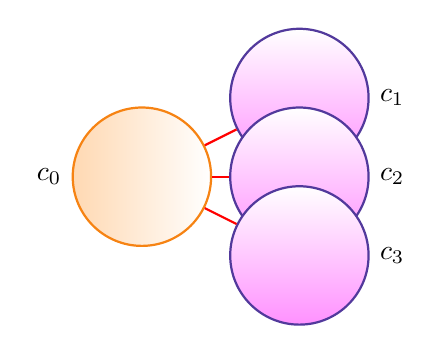
\begin{tikzpicture}[auto, thick]
  % Place base case
  \node[base,label=left:$c_0$] (base) at (0,0) {};
  
  \node[contingency,label=right:$c_1$] (c1) at (2,1) {};
  \node[contingency,label=right:$c_2$] (c2) at (2,0) {};
  \node[contingency,label=right:$c_3$] (c3) at (2,-1) {};
  
  \path[cedge] (base) edge (c1);
  \path[cedge] (base) edge (c2);
  \path[cedge] (base) edge (c3);
  
  
  
%  \foreach \place/\name in {{(0,-1)/a}, {(2,0)/b}, {(2,2)/c}, {(0,2)/d},
%           {(-2,0)/e}}
%    \node[superpeers] (\name) at \place {a};
%  \foreach \source/\dest in {a/b, a/c, a/d, b/c, c/d,a/e,d/e}
%    \path (\source) edge (\dest);
   %
   % Place normal peers
%  \foreach \pos/\i in {above left of/1, left of/2, below left of/3}
%    \node[peers, \pos = e] (e\i) {};
%   \foreach \speer/\peer in {e/e1,e/e2,e/e3}
%    \path (\speer) edge (\peer);
   %
%   \foreach \pos/\i in {above right of/1, right of/2, below right of/3}
%    \node[peers, \pos =b ] (b\i) {};
%   \foreach \speer/\peer in {b/b1,b/b2,b/b3}
%   \path (\speer) edge (\peer);
   %
%   \node[peers, above of=d] (d1){};
%   \path (d) edge (d1);
   %
%   \foreach \pos/\i in {below left of/1, below of/2}
%   \node[peers, \pos =a ] (a\i) {};
%   \foreach \speer/\peer in {a/a1,a/a2}
%   \path (\speer) edge (\peer);

\end{tikzpicture}
\caption{Contingency constrained optimal power flow example with three contingencies. $c_0$ represents the base case (or no contingency case). $c_1$, $c_2$, $c_3$ are the three contingency cases. Each of the contingency states is coupled with the base-case through ramping constraints (denoted by \textcolor{red}{red} lines)}
\label{fig:scopflow}
\end{figure}


In general form, the equations for contingency-constrained optimal power flow are given by
(\ref{eq:scopflow_start}) -- (\ref{eq:scopflow_end}). This is a two-stage
stochastic optimization problem where the first stage is the base case $c_0$ and
each of the contingency states $c_i, i \in [1,N_c]$ are second-stage
subproblems. SCOPFLOW aims to minimize the objective $\sum_{c=0}^{N_c}f(x_c)$,
while adhering to the equality $g_c(x_c)$, inequality $h_c(x_c)$, and the
lower/upper bound ($x^-$,$x^+$) constraints. Equation (\ref{eq:scopflow_end})
represents the coupling between the base-case $c_0$ and each of the contingency states
$c_i$. Equation (\ref{eq:scopflow_end}) is the most typical form of coupling
that limits the deviation of the contingency variables $x_c$ from the base $x_0$
to within $\Delta x_c$. An example of this constraint could be the allowed real power output deviation for the generators constrained by their ramp limit, which is currently the only constraint SCOPFLOW supports.


\begin{align}
\centering
\text{min}&~\sum_{c=0}^{N_c}f_c(x_c)&  \label{eq:scopflow_start}\\
&\text{s.t.}& \nonumber \\
&~g_c(x_c) = 0,                             &c \in \left[0,N_c\right]& \\
&~h_c(x_c) \le 0,                           &c \in \left[0,N_c\right]& \\
x^- & \le x_c \le x^+,                     &c\in \left[0,N_c\right]& \\
-\Delta x_c & \le x_c - x_0 \le \Delta x_c,&c \in \left[1,N_c\right]&
\label{eq:scopflow_end}
\end{align}

\subsection{Multiperiod}

In the multi-period version, each contingency is comprised of multiple time-periods. The multiple periods have variables and constraints as described in chapter \ref{chap:tcopflow}. An example of multi-contingency multi-period optimal power flow is illustrated in Fig. \ref{fig:ctopflow} for multi-period SCOPFLOW with three contingencies $c_1$, $c_2$, and $c_3$ coupled to the base case $c_0$. Each state is multi-period with two time-periods. Each time-step is coupled with its adjacent one through ramping constraints. We assume that the contingency is incident at the first time-step, i.e. at $t_0$. This results in the coupling between the contingency cases $c_i, i \in [1,N_c]$ and the base-case $c_0$ only at time-step $t_0$.

\definecolor{lavander}{cmyk}{0,0.48,0,0}
\definecolor{violet}{cmyk}{0.79,0.88,0,0}
\definecolor{burntorange}{cmyk}{0,0.52,1,0}

\def\lav{lavander!90}
\def\oran{orange!30}

\tikzstyle{contingency}=[draw,circle,violet,bottom color=\lav,
                  top color= white, text=violet,minimum width=50pt]
\tikzstyle{base}=[draw,circle,burntorange, left color=\oran,
                       text=violet,minimum width=50pt]

\tikzstyle{time}=[draw,circle,blue,text=violet,minimum width=2pt]
\tikzstyle{tbase}=[draw,circle,burntorange, left color=\oran,
                            text=violet,minimum width=2pt]
                       
\tikzstyle{cedge}=[color=red]

\begin{figure}[h!]
\centering
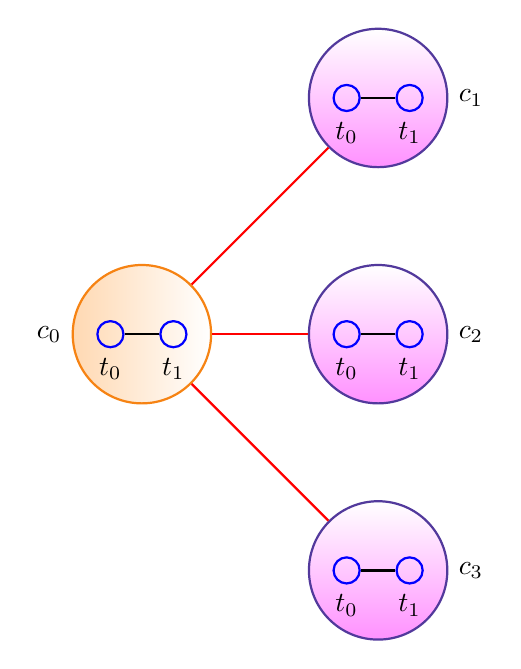
\begin{tikzpicture}[auto, thick]
  % Place base case
  \node[base,label=left:$c_0$] (base) at (0,0) {};
  \node[time,label=below:$t_0$] (c0t0) at (-0.4,0) {};
  \node[time,label=below:$t_1$] (c0t1) at (0.4,0) {};
  
  \node[contingency,label=right:$c_1$] (c1) at (3,3) {};
  \node[time,label=below:$t_0$] (c1t0) at (2.6,3) {};
  \node[time,label=below:$t_1$] (c1t1) at (3.4,3) {};

  \node[contingency,label=right:$c_2$] (c2) at (3,0) {};
  \node[time,label=below:$t_0$] (c2t0) at (2.6,0) {};
  \node[time,label=below:$t_1$] (c2t1) at (3.4,0) {};

  
  \node[contingency,label=right:$c_3$] (c3) at (3,-3) {};
  \node[time,label=below:$t_0$] (c3t0) at (2.6,-3) {};
  \node[time,label=below:$t_1$] (c3t1) at (3.4,-3) {};
  
  \path (c0t0) edge (c0t1);
  \path (c1t0) edge (c1t1);
  \path (c2t0) edge (c2t1);
  \path (c3t0) edge (c3t1);
  
  \path[cedge] (base) edge (c1);
  \path[cedge] (base) edge (c2);
  \path[cedge] (base) edge (c3);  
  
  
%  \foreach \place/\name in {{(0,-1)/a}, {(2,0)/b}, {(2,2)/c}, {(0,2)/d},
%           {(-2,0)/e}}
%    \node[superpeers] (\name) at \place {a};
%  \foreach \source/\dest in {a/b, a/c, a/d, b/c, c/d,a/e,d/e}
%    \path (\source) edge (\dest);
   %
   % Place normal peers
%  \foreach \pos/\i in {above left of/1, left of/2, below left of/3}
%    \node[peers, \pos = e] (e\i) {};
%   \foreach \speer/\peer in {e/e1,e/e2,e/e3}
%    \path (\speer) edge (\peer);
   %
%   \foreach \pos/\i in {above right of/1, right of/2, below right of/3}
%    \node[peers, \pos =b ] (b\i) {};
%   \foreach \speer/\peer in {b/b1,b/b2,b/b3}
%   \path (\speer) edge (\peer);
   %
%   \node[peers, above of=d] (d1){};
%   \path (d) edge (d1);
   %
%   \foreach \pos/\i in {below left of/1, below of/2}
%   \node[peers, \pos =a ] (a\i) {};
%   \foreach \speer/\peer in {a/a1,a/a2}
%   \path (\speer) edge (\peer);

\end{tikzpicture}
\caption{Multi-period contingency constrained optimal power flow example with two contingencies $c_0$ and $c_1$, each with two time-periods $t_0$, $t_1$. State $c_0$ represents the base case (no contingency) case. The contingency states $c_1$,$c_2$,$c_3$ are coupled with the no-contingency state $c_0$. The {\textcolor{red}{red}} line denotes the coupling between the contingencies.}
\label{fig:ctopflow}
\end{figure}


The overall objective of this contingency-constrained multi-period optimal power flow is to find a secure dispatch for base-case $c_0$ while adhering to contingency and temporal constraints. The general formulation of this problem is given in Eqs. (\ref{eq:ctopflow_start}) -- (\ref{eq:ctopflow_end}).

\begin{align}
\centering
\text{min}&~\sum_{c=0}^{N_c}\sum_{t=0}^{N_t-1}f_{ct}(x_{c,t})& \label{eq:ctopflow_start}\\
&\text{s.t.}& \nonumber \\
&~g_{ct}(x_{c,t}) = 0,                                        &c \in \left[0,N_c\right], t \in \left[0,N_t-1\right]& \\
&~h_{ct}(x_{c,t}) \le 0,                                      &c \in \left[0,N_c\right], t \in \left[0,N_t-1\right]& \\
x^- & \le x_{c,t} \le x^+,                               &c \in \left[0,N_c\right], t\in \left[0,N_t-1\right]& \\
-\Delta x_t & \le x_{c,t} - x_{c,t-\Delta{t}} \le \Delta x_t,&c \in \left[0,N_c\right], t \in \left[1,N_t-1\right]& \label{eq:ctopflow_time_coupling}\\
-\Delta x_c & \le x_{c,0} - x_{0,0} \le \Delta x_c,&c \in \left[1,N_c\right]& \\
\label{eq:ctopflow_end}
\end{align}

In this formulation, the objective is to reduce the cost for the base-case time
horizon, where $f(x_{0,t})$ is the objective cost for contingency $c_0$ at time
$t$. Equation (\ref{eq:ctopflow_end}) represents the coupling between the base
case $c_0$ and each contingency $c_i$ at time-step $t_0$. We use a simple box
constraint $\Delta x_c$ to restrict the  deviation of decision variables
$x_{c,0}$ from the base-case $x_{0,0}$. The bound $\Delta x_c$ could represent here, for example, the allowable reserve for each generator.

\section{Solvers}
\scopflow supports solving the optimization problem via \ipopt, \hiop, or \emph{EMPAR}. \ipopt can solve \scopflow on single rank only. \hiop supports solving the problem in parallel using a primal-decomposition algorithm. With HiOp, one can solve the subproblem either on the CPU or GPU by selecting the appropriate subproblem model and solver (see options table below).  However, note that \emph{ExaGO needs to be built with \ipopt even when using \hiop solver.} The \emph{EMPAR} solver does not solve the security-constrained ACOPF problem, it only solves the base-case and the contingencies independently with \opflow. It distributes the contingencies to different processes when executed in parallel.

\section{Input and Output}
To execute SCOPFLOW, the following files are required:
\begin{itemize}
    \item \textbf{Network file:} The network file describing the network details. Only \matpower format files are currently supported.
    \item \textbf{Contingency file:} The file describing the
      contingencies. Contingencies can be single or multiple
      outages. Two formats are excepted, with the format distinguished
      by file name extension.  A contingency file in PTI format must
      have a \texttt{.cont} extension.  A PSS/E format file must have
      a \texttt{.con} extension.
\end{itemize}
If the multi-period option is chosen, then additional files describing the load and wind generation can be (optionally) set.
\begin{itemize}
    \item \textbf{Load data:} One file for load real power and one for reactive power. The files need to be in CSV format. An example of the format for the 9-bus case is \href{https://gitlab.pnnl.gov/exasgd/frameworks/exago/-/tree/master/datafiles/case9}{here}.
    \item \textbf{Wind generation:} The wind generation time-series described in CSV format. See an example of the format \href{https://gitlab.pnnl.gov/exasgd/frameworks/exago/-/tree/master/datafiles/case9}{here}.
\end{itemize}

The \scopflow output is saved to a directory named \texttt{scopflowout}. This
directory contains $N_c$ files to save the solution for each contingency in
MATPOWER datafile format. Each file has the name \texttt{cont_xx} where \texttt{xx} is the contingency number. 

If the multi-period option is chosen then $N_c$ subdirectories are created (one
for each contingency), and each subdirectory contains $N_t$ output files, one
for each time-period. The subdirectories have the naming convention
\texttt{cont_xx} and the output file are named as \texttt{t_yy} where \texttt{yy} is the time-step number.

\section{Usage}

\begin{lstlisting}
  ./scopflow -netfile <netfilename> -ctgcfile <ctgcfilename> \
  <scopflowoptions> [-scopflow_enable_multiperiod 1]
\end{lstlisting}

\section{Options}
See table \ref{tab:scopflow_options}. In addition, all \opflow options in Table \ref{tab:opflow_options} and \tcopflow options in Table \ref{tab:tcopflow_options} can be used.
\begin{table}[H]
  \caption{SCOPFLOW options}
  \small
  \begin{tabular}{|p{0.3\textwidth}|p{0.2\textwidth}|p{0.3\textwidth}|p{0.2\textwidth}|}
    \hline
    \textbf{Option} & \textbf{Meaning} & \textbf{Values (Default value)} & \textbf{Compatibility} \\ \hline
    -netfile & Network file name & string $<$ 4096 characters (\href{https://gitlab.pnnl.gov/exasgd/frameworks/exago/-/blob/master/datafiles/case9/case9mod_gen3_wind.m}{case9mod\_gen3\_wind.m}) &\\ \hline
    -ctgcfile & Contingency file name & string $<$ 4096 characters (\href{https://gitlab.pnnl.gov/exasgd/frameworks/exago/-/blob/master/datafiles/case9/case9.cont}{case9.cont}) &\\ \hline
    -print\_output & Print output to screen & 0 or 1 (0) &\\ \hline
    -save\_output & Save output to directory & 0 or 1 (0) & Format determined by OPFLOW option. \\ \hline
    -scopflow\_output\_directory & Output directory path & ``scopflowout'' & \\ \hline
    -scopflow\_model & SCOPFLOW model type & GENRAMP, GENRAMPT (GENRAMP) & \\ \hline
    -scopflow\_solver & Set solver for scopflow & IPOPT, HIOP, or EMPAR (IPOPT) &\\ \hline
    -scopflow\_subproblem\_solver & Set solver for subproblem & IPOPT or HIOP (IPOPT) &Only when using HiOp solver for SCOPFLOW \\ \hline
    -scopflow\_subproblem\_model & Set model for subproblem & See OPFLOW chapter &Only when using HiOp solver for SCOPFLOW \\ \hline
    -scopflow\_Nc & Number of contingencies & int (0. Passing -1 results in all contingencies in the file used) &\\ \hline
    -scopflow\_mode & Operation mode: Preventive or corrective & 0 or 1 (0) &\\ \hline
    -scopflow\_enable\_multiperiod & Multi-period SCOPFLOW & 0 or 1 (0) & IPOPT solver only\\ \hline
    -scopflow\_ploadprofile & Real power load profile & string (\href{https://gitlab.pnnl.gov/exasgd/frameworks/exago/-/blob/master/datafiles/case9/load_P.csv}{load\_P.csv}) &\\ \hline
    -scopflow\_qloadprofile & Reactive power load profile & string (\href{https://gitlab.pnnl.gov/exasgd/frameworks/exago/-/blob/master/datafiles/case9/load_Q.csv}{load\_Q.csv}) &\\ \hline
    -scopflow\_windgenprofile & Wind generation profile & string (\href{https://gitlab.pnnl.gov/exasgd/frameworks/exago/-/blob/master/datafiles/case9/scenarios_9bus.csv}{case9/scenarios\_9bus.csv}) &\\ \hline
    -scopflow\_dT & Length of time-step (minutes) & double (5.0) &\\ \hline
    -scopflow\_duration & Total duration (hours) & double (0.5) &\\ \hline 
    -scopflow\_tolerance & Optimization solver tolerance & double (1e-6) &\\ \hline 
  \end{tabular}
  \label{tab:scopflow_options}
\end{table}

Depending on the value chosen for \texttt{-scopflow_mode}, SCOPFLOW can operate
either in \emph{preventive} (mode = 0) or \emph{corrective} (mode = 1) mode. In
the preventive mode, the PV and PQ generator real power is fixed to its
corresponding base-case values. The generators at the reference bus pick up any
make-up power required for the contingency. The corrective mode allows deviation
of the PV and PQ generator real power from the base-case dispatch constrained by
its 30-min. ramp rate capability. The optimization decides the optimal
redispatch. One can have AGC control instead of having the generators proportionally share the deficit/excess power by using the option \emph(-opflow_use_agc).

The option \texttt{-scopflow_enable_multiperiod} 1 must be used in order to enable any of the options listed in table \ref{tab:scopflow_options} for multiperiod analysis.

\section{Examples}

Some \scopflow example runs are provided with some sample output. Options are the default options given in table \ref{tab:opflow_options}, \ref{tab:tcopflow_options} and \ref{tab:scopflow_options} unless otherwise specified. Sample output is generated by running examples in the installation directory.

Example using the \ipopt solver:

\begin{lstlisting}
./bin/scopflow -netfile $EXAGO_DIR/datafiles/case9/case9mod.m -ctgcfile $EXAGO_DIR/datafiles/case9/case9.cont -scopflow_Nc 4 -scopflow_solver IPOPT -print_output 
[ExaGO] SCOPFLOW: Application created
[ExaGO] SCOPFLOW running with 5 subproblems (base case + 4 contingencies)
[ExaGO] SCOPFLOW: Using IPOPT solver
[ExaGO] SCOPFLOW: Setup completed

******************************************************************************
This program contains Ipopt, a library for large-scale nonlinear optimization.
 Ipopt is released as open source code under the Eclipse Public License (EPL).
         For more information visit http://projects.coin-or.org/Ipopt
******************************************************************************

This is Ipopt version 3.12.10, running with linear solver ma27.

Number of nonzeros in equality constraint Jacobian...:      598
Number of nonzeros in inequality constraint Jacobian.:      328
Number of nonzeros in Lagrangian Hessian.............:      660

Total number of variables............................:      144
                     variables with only lower bounds:        0
                variables with lower and upper bounds:      104
                     variables with only upper bounds:        0
Total number of equality constraints.................:      114
Total number of inequality constraints...............:       82
        inequality constraints with only lower bounds:        0
   inequality constraints with lower and upper bounds:       82
        inequality constraints with only upper bounds:        0

iter    objective    inf_pr   inf_du lg(mu)  ||d||  lg(rg) alpha_du alpha_pr  ls
   0  1.0318125e+04 1.80e+00 1.00e+02  -1.0 0.00e+00    -  0.00e+00 0.00e+00   0
   1  9.2868867e+03 1.56e+00 8.62e+01  -1.0 1.08e+00    -  6.27e-01 1.31e-01f  1
   2  9.0292788e+03 1.50e+00 3.50e+02  -1.0 2.60e+00    -  1.37e-03 4.28e-02f  1
   3  6.8151659e+03 9.02e-01 3.07e+03  -1.0 1.03e+00    -  4.57e-02 4.09e-01f  1
   4  5.6911245e+03 5.63e-01 2.09e+03  -1.0 7.85e-01   2.0 1.22e-01 3.87e-01f  1
   5  5.6219674e+03 5.39e-01 2.00e+03  -1.0 8.34e-01    -  1.99e-01 4.29e-02f  1
   6  4.7820782e+03 2.34e-01 7.42e+02  -1.0 7.27e-01    -  5.45e-01 5.75e-01f  1
   7  4.1986838e+03 3.84e-02 2.59e+02  -1.7 4.11e-01    -  3.64e-01 1.00e+00f  1
   8  4.1593634e+03 6.26e-02 1.52e+01  -1.7 3.77e-01    -  5.76e-01 1.00e+00f  1
   9  4.1598457e+03 3.63e-04 1.53e+00  -2.5 4.57e-02   1.5 8.25e-01 1.00e+00h  1
iter    objective    inf_pr   inf_du lg(mu)  ||d||  lg(rg) alpha_du alpha_pr  ls
  10  4.1472241e+03 4.61e-02 5.44e+00  -3.8 1.15e-01    -  3.15e-01 1.00e+00f  1
  11  4.1437514e+03 3.32e-02 3.50e+00  -3.8 1.95e-01    -  5.75e-01 3.47e-01h  1
  12  4.1440398e+03 1.07e-02 1.64e+00  -3.8 7.68e-02    -  2.42e-01 6.18e-01h  1
  13  4.1444455e+03 1.33e-03 4.38e-02  -3.8 3.29e-02    -  9.49e-01 1.00e+00h  1
  14  4.1444954e+03 5.41e-06 2.57e-02  -3.8 2.31e-03   1.0 1.00e+00 1.00e+00h  1
  15  4.1444778e+03 1.47e-05 1.41e-02  -3.8 3.80e-03   0.6 1.00e+00 1.00e+00h  1
  16  4.1444804e+03 1.82e-05 4.42e-03  -3.8 3.58e-03   0.1 1.00e+00 1.00e+00h  1
  17  4.1444799e+03 9.05e-05 3.06e-03  -3.8 7.43e-03  -0.4 1.00e+00 1.00e+00h  1
  18  4.1444616e+03 1.08e-05 5.76e-03  -5.7 3.72e-03  -0.9 1.00e+00 9.26e-01h  1
  19  4.1444608e+03 5.66e-06 1.11e-04  -5.7 2.43e-03  -1.3 1.00e+00 1.00e+00h  1
iter    objective    inf_pr   inf_du lg(mu)  ||d||  lg(rg) alpha_du alpha_pr  ls
  20  4.1444608e+03 2.21e-08 3.62e-05  -5.7 2.38e-03  -1.8 1.00e+00 1.00e+00H  1
  21  4.1444608e+03 3.35e-07 2.93e-05  -5.7 5.76e-03  -2.3 1.00e+00 1.00e+00H  1
  22  4.1444608e+03 2.25e-04 1.95e-05  -5.7 1.15e-02  -2.8 1.00e+00 1.00e+00h  1
  23  4.1444608e+03 5.41e-04 1.11e-05  -5.7 1.96e-02  -3.2 1.00e+00 1.00e+00h  1
  24  4.1444608e+03 2.03e-02 1.22e-04  -5.7 1.15e-01  -3.7 1.00e+00 1.00e+00h  1
  25  4.1444608e+03 8.07e-04 2.02e-05  -5.7 2.32e-02  -3.3 1.00e+00 1.00e+00h  1
  26  4.1444608e+03 6.02e-03 3.97e-05  -5.7 6.75e-02  -3.8 1.00e+00 1.00e+00h  1
  27  4.1444608e+03 1.93e-02 1.75e-04  -5.7 1.17e-01  -4.3 1.00e+00 1.00e+00h  1
  28  4.1444608e+03 4.88e-02 7.07e-05  -5.7 1.71e-01  -4.7 1.00e+00 1.00e+00h  1
  29  4.1444608e+03 8.42e-04 6.07e-06  -5.7 3.53e-02  -4.3 1.00e+00 1.00e+00h  1
iter    objective    inf_pr   inf_du lg(mu)  ||d||  lg(rg) alpha_du alpha_pr  ls
  30  4.1444608e+03 1.16e-02 4.10e-06  -5.7 1.11e-01  -4.8 1.00e+00 1.00e+00h  1
  31  4.1444608e+03 1.54e-03 1.71e-06  -5.7 3.87e-02  -4.4 1.00e+00 1.00e+00h  1
  32  4.1444608e+03 2.12e-02 9.93e-06  -5.7 1.38e-01  -4.8 1.00e+00 1.00e+00h  1
  33  4.1444608e+03 1.52e-01 8.57e-05  -5.7 5.25e-01  -5.3 1.00e+00 1.00e+00h  1
  34  4.1444608e+03 5.89e-03 2.06e-05  -5.7 1.27e-01  -4.9 1.00e+00 1.00e+00h  1
  35  4.1444608e+03 2.60e-01 1.06e-04  -5.7 1.23e+00    -  7.38e-01 1.00e+00H  1
  36  4.1444608e+03 4.78e-02 3.16e-05  -5.7 3.18e-01    -  1.00e+00 1.00e+00h  1
  37  4.1444608e+03 1.18e-03 3.22e-07  -5.7 7.50e-02    -  1.00e+00 1.00e+00h  1
  38  4.1444608e+03 3.36e-05 2.96e-09  -5.7 1.62e-02    -  1.00e+00 1.00e+00h  1
  39  4.1444608e+03 3.14e-10 5.68e-13  -5.7 5.87e-05    -  1.00e+00 1.00e+00h  1
iter    objective    inf_pr   inf_du lg(mu)  ||d||  lg(rg) alpha_du alpha_pr  ls
  40  4.1444605e+03 7.54e-08 1.83e-07  -7.0 2.81e-04    -  1.00e+00 1.00e+00h  1

Number of Iterations....: 40

                                   (scaled)                 (unscaled)
Objective...............:   9.2925124417578417e+01    4.1444605490239974e+03
Dual infeasibility......:   1.8347495281748061e-07    8.1829828956596351e-06
Constraint violation....:   1.3290786859965209e-08    1.3290786859965209e-08
Complementarity.........:   2.6885276874539710e-07    1.1990833486044711e-05
Overall NLP error.......:   2.6885276874539710e-07    1.1990833486044711e-05


Number of objective function evaluations             = 44
Number of objective gradient evaluations             = 41
Number of equality constraint evaluations            = 44
Number of inequality constraint evaluations          = 44
Number of equality constraint Jacobian evaluations   = 41
Number of inequality constraint Jacobian evaluations = 41
Number of Lagrangian Hessian evaluations             = 40
Total CPU secs in IPOPT (w/o function evaluations)   =      0.078
Total CPU secs in NLP function evaluations           =      0.026

EXIT: Optimal Solution Found.
=============================================================
Security-Constrained Optimal Power Flow
=============================================================
Number of contingencies             4
Multi-period contingencies?         NO
Solver                              IPOPT
Initialization                      MIDPOINT
Load loss allowed                   NO
Power imbalance allowed             NO
Ignore line flow constraints        NO


Convergence status                  CONVERGED
Objective value (base)              4144.46

----------------------------------------------------------------------
Bus        Pd      Qd      Vm      Va      mult_Pmis      mult_Qmis      Pslack         Qslack        
----------------------------------------------------------------------
1         0.00    0.00   1.100   0.000      2102.91         0.00         0.00         0.00
2         0.00    0.00   1.095   3.928      2059.18        -0.00         0.00         0.00
3         0.00    0.00   1.087   2.120      2065.15        -0.00         0.00         0.00
4         0.00    0.00   1.097  -1.993      2103.17         0.08         0.00         0.00
5        75.00   50.00   1.079  -3.060      2113.46         7.29         0.00         0.00
6        90.00   30.00   1.087  -3.927      2129.85         1.62         0.00         0.00
7         0.00    0.00   1.100   0.535      2059.57        -0.04         0.00         0.00
8       100.00   35.00   1.089  -1.720      2079.34         2.99         0.00         0.00
9         0.00    0.00   1.100  -0.135      2065.43        -0.09         0.00         0.00

----------------------------------------------------------------------------------------
From       To       Status     Sft      Stf     Slim     mult_Sf  mult_St 
----------------------------------------------------------------------------------------
1          4          1       73.18    72.98   380.00    -0.00    -0.00
2          7          1      114.18   114.68   250.00    -0.00    -0.00
3          9          1       83.58    84.61   300.00    -0.00    -0.00
4          5          1       29.69    40.50   250.00    -0.00    -0.00
4          6          1       44.86    46.03   250.00    -0.00    -0.00
5          7          1       51.29    49.04   250.00    -0.00    -0.00
6          9          1       48.94    51.43   150.00    -0.00    -0.00
7          8          1       66.61    68.11   250.00    -0.00    -0.00
8          9          1       38.87    34.15   150.00    -0.00    -0.00

----------------------------------------------------------------------------------------
Gen      Status     Fuel     Pg       Qg       Pmin     Pmax     Qmin     Qmax  
----------------------------------------------------------------------------------------
1          1    UNDEFINED    72.86     6.79    10.00   350.00  -300.00   300.00
2          1    UNDEFINED   114.07    -5.13    10.00   300.00  -300.00   300.00
3          1    UNDEFINED    80.21   -23.48    10.00   270.00  -300.00   300.00
[ExaGO] Finalizing scopflow application.
\end{lstlisting}

Example using HiOp solver with Ipopt as the subproblem solver.
\begin{lstlisting}
bin/scopflow -netfile $EXAGO_DIR/datafiles/case9/case9mod.m -ctgcfile $EXAGO_DIR/datafiles/case9/case9.cont -scopflow_Nc 4 -scopflow_solver IPOPT -print_output -scopflow_solver HIOP -scopflow_subproblem_solver IPOPT -scopflow_subproblem_model POWER_BALANCE_POLAR
[ExaGO] SCOPFLOW: Application created
[ExaGO] SCOPFLOW running with 5 subproblems (base case + 4 contingencies)
[ExaGO] SCOPFLOW: Using HIOP solver
Failed to read option file 'hiop_pridec.options'. Hiop will use default options.
[ExaGO] SCOPFLOW: Setup completed
total number of recourse problems  4

******************************************************************************
This program contains Ipopt, a library for large-scale nonlinear optimization.
 Ipopt is released as open source code under the Eclipse Public License (EPL).
         For more information visit http://projects.coin-or.org/Ipopt
******************************************************************************

This is Ipopt version 3.12.10, running with linear solver ma27.

Number of nonzeros in equality constraint Jacobian...:      114
Number of nonzeros in inequality constraint Jacobian.:       72
Number of nonzeros in Lagrangian Hessian.............:       96

Total number of variables............................:       24
                     variables with only lower bounds:        0
                variables with lower and upper bounds:       16
                     variables with only upper bounds:        0
Total number of equality constraints.................:       18
Total number of inequality constraints...............:       18
        inequality constraints with only lower bounds:        0
   inequality constraints with lower and upper bounds:       18
        inequality constraints with only upper bounds:        0

iter    objective    inf_pr   inf_du lg(mu)  ||d||  lg(rg) alpha_du alpha_pr  ls
   0  1.0318125e+04 1.80e+00 1.00e+02  -1.0 0.00e+00    -  0.00e+00 0.00e+00   0
   1  7.7157691e+03 1.17e+00 1.03e+02  -1.0 1.08e+00    -  6.27e-01 3.50e-01f  1
   2  7.6608235e+03 1.15e+00 1.01e+02  -1.0 6.28e+00    -  1.20e-02 1.37e-02f  1
   3  7.4466686e+03 1.09e+00 3.06e+02  -1.0 3.74e+00    -  4.15e-03 5.81e-02f  1
   4  5.4292675e+03 3.92e-01 4.83e+03  -1.0 7.34e-01    -  3.34e-03 6.40e-01f  1
   5  4.5792834e+03 2.24e-01 1.51e+03  -1.0 6.46e-01   2.0 8.77e-03 7.37e-01f  1
   6  4.2907579e+03 1.20e-02 3.57e+02  -1.0 3.36e-01    -  5.37e-01 1.00e+00f  1
   7  4.1690456e+03 4.40e-02 5.31e+01  -1.0 3.31e-01    -  9.22e-01 1.00e+00f  1
   8  4.1687926e+03 4.88e-04 1.93e+00  -1.0 4.79e-02   1.5 1.00e+00 1.00e+00h  1
   9  4.1497176e+03 1.19e-02 9.92e+00  -2.5 1.87e-01    -  8.38e-01 1.00e+00f  1
iter    objective    inf_pr   inf_du lg(mu)  ||d||  lg(rg) alpha_du alpha_pr  ls
  10  4.1463942e+03 1.09e-02 5.09e-01  -2.5 1.15e-01    -  8.71e-01 1.00e+00h  1
  11  4.1449657e+03 1.47e-03 1.79e-02  -2.5 2.75e-02    -  1.00e+00 1.00e+00h  1
  12  4.1445415e+03 6.63e-04 9.12e-02  -3.8 1.48e-02    -  1.00e+00 6.30e-01h  1
  13  4.1444705e+03 3.43e-04 4.96e-02  -3.8 2.08e-02    -  1.00e+00 8.93e-01h  1
  14  4.1444809e+03 4.48e-05 1.79e-04  -3.8 6.82e-03    -  1.00e+00 1.00e+00f  1
  15  4.1444611e+03 1.96e-05 4.55e-03  -5.7 4.57e-03    -  1.00e+00 9.34e-01h  1
  16  4.1444607e+03 6.49e-06 1.17e-05  -5.7 2.60e-03    -  1.00e+00 1.00e+00h  1
  17  4.1444605e+03 1.19e-06 2.07e-06  -7.0 1.11e-03    -  1.00e+00 1.00e+00h  1
  18  4.1444605e+03 1.58e-07 3.29e-07  -7.0 4.06e-04    -  1.00e+00 1.00e+00h  1

Number of Iterations....: 18

                                   (scaled)                 (unscaled)
Objective...............:   9.2925122354655841e+01    4.1444604570176507e+03
Dual infeasibility......:   3.2927387965389691e-07    1.4685615032563802e-05
Constraint violation....:   2.6639677713768961e-08    2.6639677713768961e-08
Complementarity.........:   4.7840038622596930e-07    2.1336657225678232e-05
Overall NLP error.......:   4.7840038622596930e-07    2.1336657225678232e-05


Number of objective function evaluations             = 19
Number of objective gradient evaluations             = 19
Number of equality constraint evaluations            = 19
Number of inequality constraint evaluations          = 19
Number of equality constraint Jacobian evaluations   = 19
Number of inequality constraint Jacobian evaluations = 19
Number of Lagrangian Hessian evaluations             = 18
Total CPU secs in IPOPT (w/o function evaluations)   =      0.027
Total CPU secs in NLP function evaluations           =      0.002

EXIT: Optimal Solution Found.
This is Ipopt version 3.12.10, running with linear solver ma27.

Number of nonzeros in equality constraint Jacobian...:      118
Number of nonzeros in inequality constraint Jacobian.:       64
Number of nonzeros in Lagrangian Hessian.............:      141

Total number of variables............................:       30
                     variables with only lower bounds:        0
                variables with lower and upper bounds:       22
                     variables with only upper bounds:        0
Total number of equality constraints.................:       24
Total number of inequality constraints...............:       16
        inequality constraints with only lower bounds:        0
   inequality constraints with lower and upper bounds:       16
        inequality constraints with only upper bounds:        0

iter    objective    inf_pr   inf_du lg(mu)  ||d||  lg(rg) alpha_du alpha_pr  ls
   0  0.0000000e+00 1.80e+00 0.00e+00  -1.0 0.00e+00    -  0.00e+00 0.00e+00   0
   1  0.0000000e+00 1.41e+00 3.55e+01  -1.0 9.96e-01    -  6.48e-01 2.16e-01h  1
   2  0.0000000e+00 1.36e+00 5.74e+01  -1.0 3.86e+00    -  3.79e-03 3.37e-02f  1
   3  0.0000000e+00 1.12e+00 3.23e+02  -1.0 1.01e+00    -  1.98e-02 1.76e-01f  1
   4  0.0000000e+00 4.03e-01 7.31e+02  -1.0 7.32e-01    -  2.71e-02 9.03e-01f  1
   5  0.0000000e+00 8.41e-02 1.58e+02  -1.0 6.95e-01    -  4.70e-01 8.52e-01h  1
   6  0.0000000e+00 4.93e-03 3.36e+01  -1.0 1.85e-01    -  1.00e+00 1.00e+00f  1
   7  0.0000000e+00 2.20e-02 2.50e+01  -1.0 6.50e-01    -  4.45e-01 2.50e-01h  3
   8  0.0000000e+00 1.07e-01 5.13e+00  -1.0 3.57e-01   0.0 1.00e+00 1.00e+00h  1
   9  0.0000000e+00 1.07e-01 4.86e+00  -1.7 9.45e-01    -  3.30e-01 1.98e-01h  2
iter    objective    inf_pr   inf_du lg(mu)  ||d||  lg(rg) alpha_du alpha_pr  ls
  10  0.0000000e+00 9.21e-03 3.47e+00  -1.7 1.17e-01  -0.5 8.84e-01 1.00e+00h  1
  11  0.0000000e+00 2.70e-02 9.88e-01  -1.7 1.67e-01    -  1.00e+00 1.00e+00h  1
  12  0.0000000e+00 8.46e-03 1.62e-01  -1.7 1.58e-01  -1.0 1.00e+00 1.00e+00h  1
  13  0.0000000e+00 7.11e-04 1.09e-01  -2.5 4.58e-02  -1.4 1.00e+00 1.00e+00h  1
  14  0.0000000e+00 1.11e-01 9.70e-02  -2.5 1.43e+00    -  1.00e+00 1.00e+00H  1
  15  0.0000000e+00 2.40e-02 5.99e-02  -2.5 2.27e-01  -1.9 1.00e+00 1.00e+00h  1
  16  0.0000000e+00 3.45e-02 2.41e-01  -2.5 3.69e-01    -  5.82e-01 1.00e+00h  1
  17  0.0000000e+00 1.85e-02 1.46e-01  -2.5 3.58e-01    -  1.00e+00 1.00e+00h  1
  18  0.0000000e+00 8.37e-03 2.78e-02  -2.5 9.85e-02    -  1.00e+00 1.00e+00h  1
  19  0.0000000e+00 6.33e-06 5.45e-04  -3.8 6.81e-03    -  1.00e+00 1.00e+00h  1
iter    objective    inf_pr   inf_du lg(mu)  ||d||  lg(rg) alpha_du alpha_pr  ls
  20  0.0000000e+00 1.42e-07 2.95e-06  -5.7 1.02e-03    -  1.00e+00 1.00e+00h  1
  21  0.0000000e+00 1.44e-06 1.25e-07  -7.0 3.43e-03    -  1.00e+00 1.00e+00h  1

Number of Iterations....: 21

                                   (scaled)                 (unscaled)
Objective...............:   0.0000000000000000e+00    0.0000000000000000e+00
Dual infeasibility......:   1.2466133995485293e-07    1.2466133995485293e-07
Constraint violation....:   1.8383034489088956e-07    1.8383034489088956e-07
Complementarity.........:   1.0156847334169061e-07    1.0156847334169061e-07
Overall NLP error.......:   1.8383034489088956e-07    1.8383034489088956e-07


Number of objective function evaluations             = 28
Number of objective gradient evaluations             = 22
Number of equality constraint evaluations            = 28
Number of inequality constraint evaluations          = 28
Number of equality constraint Jacobian evaluations   = 22
Number of inequality constraint Jacobian evaluations = 22
Number of Lagrangian Hessian evaluations             = 21
Total CPU secs in IPOPT (w/o function evaluations)   =      0.032
Total CPU secs in NLP function evaluations           =      0.003

EXIT: Optimal Solution Found.

...
...

=============================================================
Security-Constrained Optimal Power Flow
=============================================================
Number of contingencies             4
Multi-period contingencies?         NO
Solver                              HIOP
Initialization                      MIDPOINT
Load loss allowed                   NO
Power imbalance allowed             NO
Ignore line flow constraints        NO


Convergence status                  CONVERGED
Objective value (base)              4144.46

----------------------------------------------------------------------
Bus        Pd      Qd      Vm      Va      mult_Pmis      mult_Qmis      Pslack         Qslack        
----------------------------------------------------------------------
1         0.00    0.00   1.100   0.000      2102.91         0.00         0.00         0.00
2         0.00    0.00   1.095   3.928      2059.18        -0.00         0.00         0.00
3         0.00    0.00   1.087   2.120      2065.15        -0.00         0.00         0.00
4         0.00    0.00   1.097  -1.993      2103.16         0.08         0.00         0.00
5        75.00   50.00   1.079  -3.060      2113.45         7.29         0.00         0.00
6        90.00   30.00   1.087  -3.927      2129.85         1.62         0.00         0.00
7         0.00    0.00   1.100   0.535      2059.57        -0.04         0.00         0.00
8       100.00   35.00   1.089  -1.720      2079.34         2.99         0.00         0.00
9         0.00    0.00   1.100  -0.135      2065.43        -0.09         0.00         0.00

----------------------------------------------------------------------------------------
From       To       Status     Sft      Stf     Slim     mult_Sf  mult_St 
----------------------------------------------------------------------------------------
1          4          1       73.18    72.98   380.00    -0.00    -0.00
2          7          1      114.18   114.68   250.00    -0.00    -0.00
3          9          1       83.57    84.60   300.00    -0.00    -0.00
4          5          1       29.68    40.50   250.00    -0.00    -0.00
4          6          1       44.86    46.03   250.00    -0.00    -0.00
5          7          1       51.29    49.04   250.00    -0.00    -0.00
6          9          1       48.94    51.43   150.00    -0.00    -0.00
7          8          1       66.61    68.11   250.00    -0.00    -0.00
8          9          1       38.86    34.15   150.00    -0.00    -0.00

----------------------------------------------------------------------------------------
Gen      Status     Fuel     Pg       Qg       Pmin     Pmax     Qmin     Qmax  
----------------------------------------------------------------------------------------
1          1    UNDEFINED    72.86     6.79    10.00   350.00  -300.00   300.00
2          1    UNDEFINED   114.07    -5.13    10.00   300.00  -300.00   300.00
3          1    UNDEFINED    80.21   -23.47    10.00   270.00  -300.00   300.00
[ExaGO] Finalizing scopflow application.
\end{lstlisting}
